
\title{Image Enhancement Techniques for Underwater Images}
\author{Malin Kildal}
\date{\today}

\documentclass[11pt]{article}

\usepackage{graphicx}
\usepackage{color}
\usepackage{caption}
\usepackage{subcaption}
\usepackage{url}


\makeatletter % Set distance from top of page to first float
\setlength{\@fptop}{5pt}
\makeatother


\begin{document}
\maketitle
\newpage

\begin{abstract}
This report discusses how how to improve underwater images of salmon. This is a relevant problem for the salmon breeding industry, as further image processing could be used to measure the size and weight of the fish. It could also be an opportunity to detect sick fish.

The main focus of this study is to remove irrelevant data from the image, while preserving the main object.
The image material will be both 2D and 3D, and the goal is for the size measurements to be more accurate after this image processing than before.

The report will show different image processing techniques that can be used to remove particles and noise. To measure the weight of the fish, both length, height and thickness measurements are needed. To achieve accurate measurements the result should be a clear image, where the depth measurements shows a smooth surface on the fish.

\end{abstract}
\clearpage


\tableofcontents
\clearpage


\section{Introduction}\label{introduction}

\subsection{Motivation}\label{motivation}
The work done in this report is done in cooperation with Sensomar SEALAB.
Sensomar SEALAB is a company developing camera systems for underwater use. Most of this is planned to be used in the fishing industry, especially aimed towards salmon breeding industry. The company's current goal is to be able to automatically measure the size and weight of the salmon underwater. For this goal to be reached, SEALAB uses some of the best cameras available, that has very high resolution and a very accurate depth measurement. But, due to all particles in the water, other fish in the background and light reflections, it is still not possible to use the data directly to find accurate measurements of the fish. They therefore need to both detect the fish, to be able to take a good photo, and they will need quite a bit of image processing on that image to remove all irrelevant data before they can find the measurements of the fish. 

With the use of image processing for noise and particle removal, it is reasonable to believe that the size measurements of the fish could be improved.

This report will show relevant background study with explanations to the different techniques that have been tried out. It will show implementation and results from different approaches. All image processing done throughout this project is done through the use of C++ and OpenCV library. OpenCV (Open Source Computer Vision) is a library of programming functions mainly aimed at real-time computer vision. \footnote{https://en.wikipedia.org/wiki/OpenCV}

\subsection{Image processing simple intro??}

\subsection{Camera used??}

\clearpage

\section{Overview of Literature}\label{overview}
This section presents background information on digital image processing, both background studies to experimental algorithms and already existing solutions. There has not been any suggestions from the literature on how to solve the exact problem of underwater depthmap images, but there are many different approaches that solves parts of the problem.
Below follows different methods containing theory and solutions for image enhancement on 2D color images and for depthmap images.


{\color{red}Do some reading on: Template matching, color interpolation, color detection}


\subsection{Filtering in the Spatial Domain}

Filtering is a technique for enhancing or modifying an image. It is used to highlight or remove certain features in an image, or both. Different techniques include smoothing, sharpening and edge enhancement. 
Filtering is a neighborhood operation, meaning that each pixels value is determined by the values of the neighboring pixels. The algorithms run though each pixel in the image and replaces the value with some value determined by the filter matrix. The matrix holding the filter is called the kernel, and the kernel size determines how big the neighborhood of the filtering will be. Filters where the output pixel is a linear combination of the values in the input pixels neighborhood is called linear filters. Averaging filter is an example of a linear filter.

For example an image containing the intensity values: 
$\begin{bmatrix}
    2 & 4 & 5 & 7 \\
    3 & 1 & 6 & 6 \\
    3 & 3 & 7 & 8 \\
    5 & 4 & 8 & 9 
\end{bmatrix}$
We want to smooth the image with an averaging filter with kernel size 3. The kernel is: 
$\frac{1}{9} \times 
\begin{bmatrix}
    1 & 1 & 1 \\
    1 & 1 & 1 \\
    1 & 1 & 1 \\
\end{bmatrix}$
Here every neighboring pixel is equally weighted, and the pixel in the center of the kernel will get the average value of all the pixels in the neighborhood. That means that if the kernel is placed in the upper left corner of the image, with the pixel with value 1 as the center pixel, the algorithm will assign the center pixel value 4, since 4 is the average value of the neighboring pixels.
This filter is good for blurring out irrelevant information, for example when wanting a smooth background.
When dealing with multi-channel images, each channel is normally processed independently.

Some other filters are explained below.


\subsubsection{Median Filter}
The median filter is a nonlinear digital filtering technique used to remove noise while preserving edges in images. The median filter algorithm runs through each pixel in the image and replaces the value with the median of neighboring pixel values. The neighboring pixels is located in a square neighborhood around the evaluated pixel. Each channel of a multi-channel image is processed independently. 

\begin{figure}[h]
    \centering
    \begin{subfigure}{0.5\textwidth}
        \centering
        \includegraphics[width=.9\linewidth]{images/literature/original_fish_image}
        \caption{Original Image}
    \end{subfigure}%
    \begin{subfigure}{.5\textwidth}
        \centering
        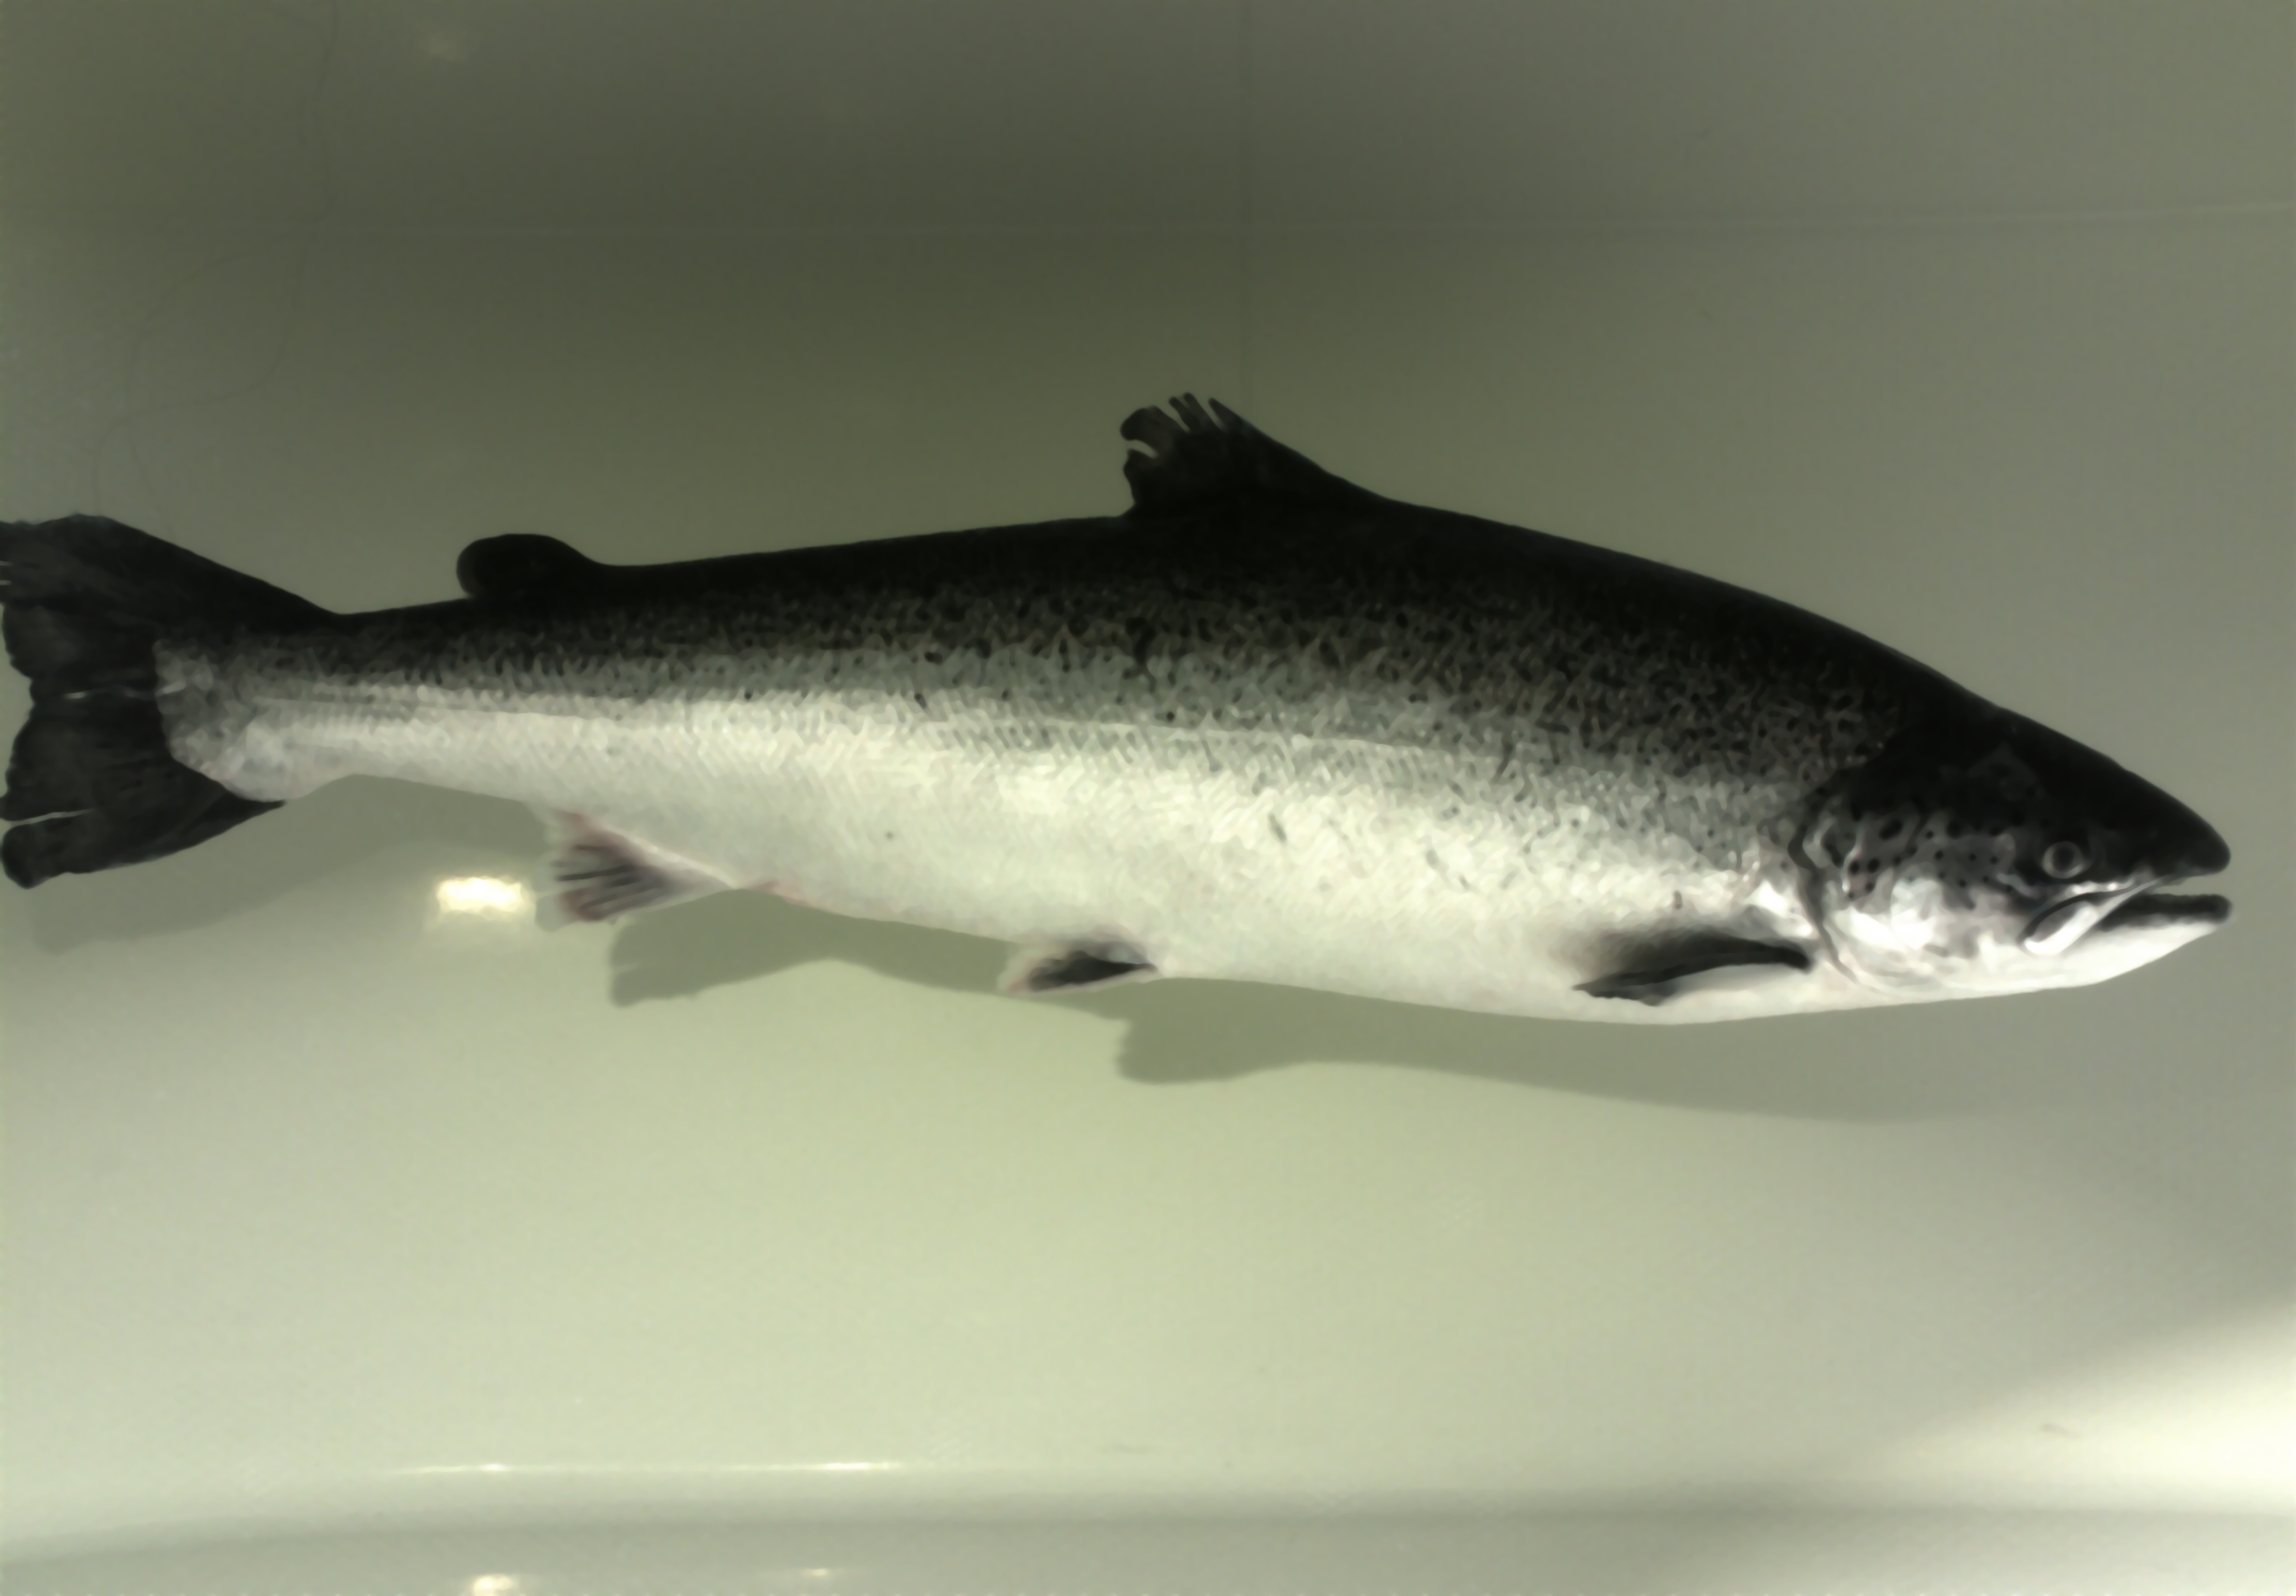
\includegraphics[width=.9\linewidth]{images/literature/median_filter}
        \caption{Median Filter}
    \end{subfigure}
    \caption{Example of median filtering}
    \label{fig:median_filter}
\end{figure}

It is seen from the images in figure \ref{fig:median_filter} that both the background and the black dots on the fish are smoothed out but the edges are preserved. Small particles is also removed; for example it is possible to see that the white particle under the fish is gone. The median filter used on this image has kernel size 9, and it was filtered four times in a row. When filtering several times in a row instead of increasing the kernel size the image will not get as blurry and small particles will still be removed.


\subsubsection{Bilateral Filter}
The bilateral filter is, just as the median filter, a nonlinear digital filter used to remove noise, while preserving sharp edges. Each pixel in an image is replaced by a weighted average of intensity values from neighboring pixels. The weight does not only depend on distance, but also on the radiometric differences such as color intensity or depth distance. 

{\color{red}Add bilateral image instead of median filter image}

\begin{figure}[h]
    \centering
    \begin{subfigure}{0.5\textwidth}
        \centering
        \includegraphics[width=.9\linewidth]{images/literature/original_fish_image}
        \caption{Original Image}
    \end{subfigure}%
    \begin{subfigure}{.5\textwidth}
        \centering
        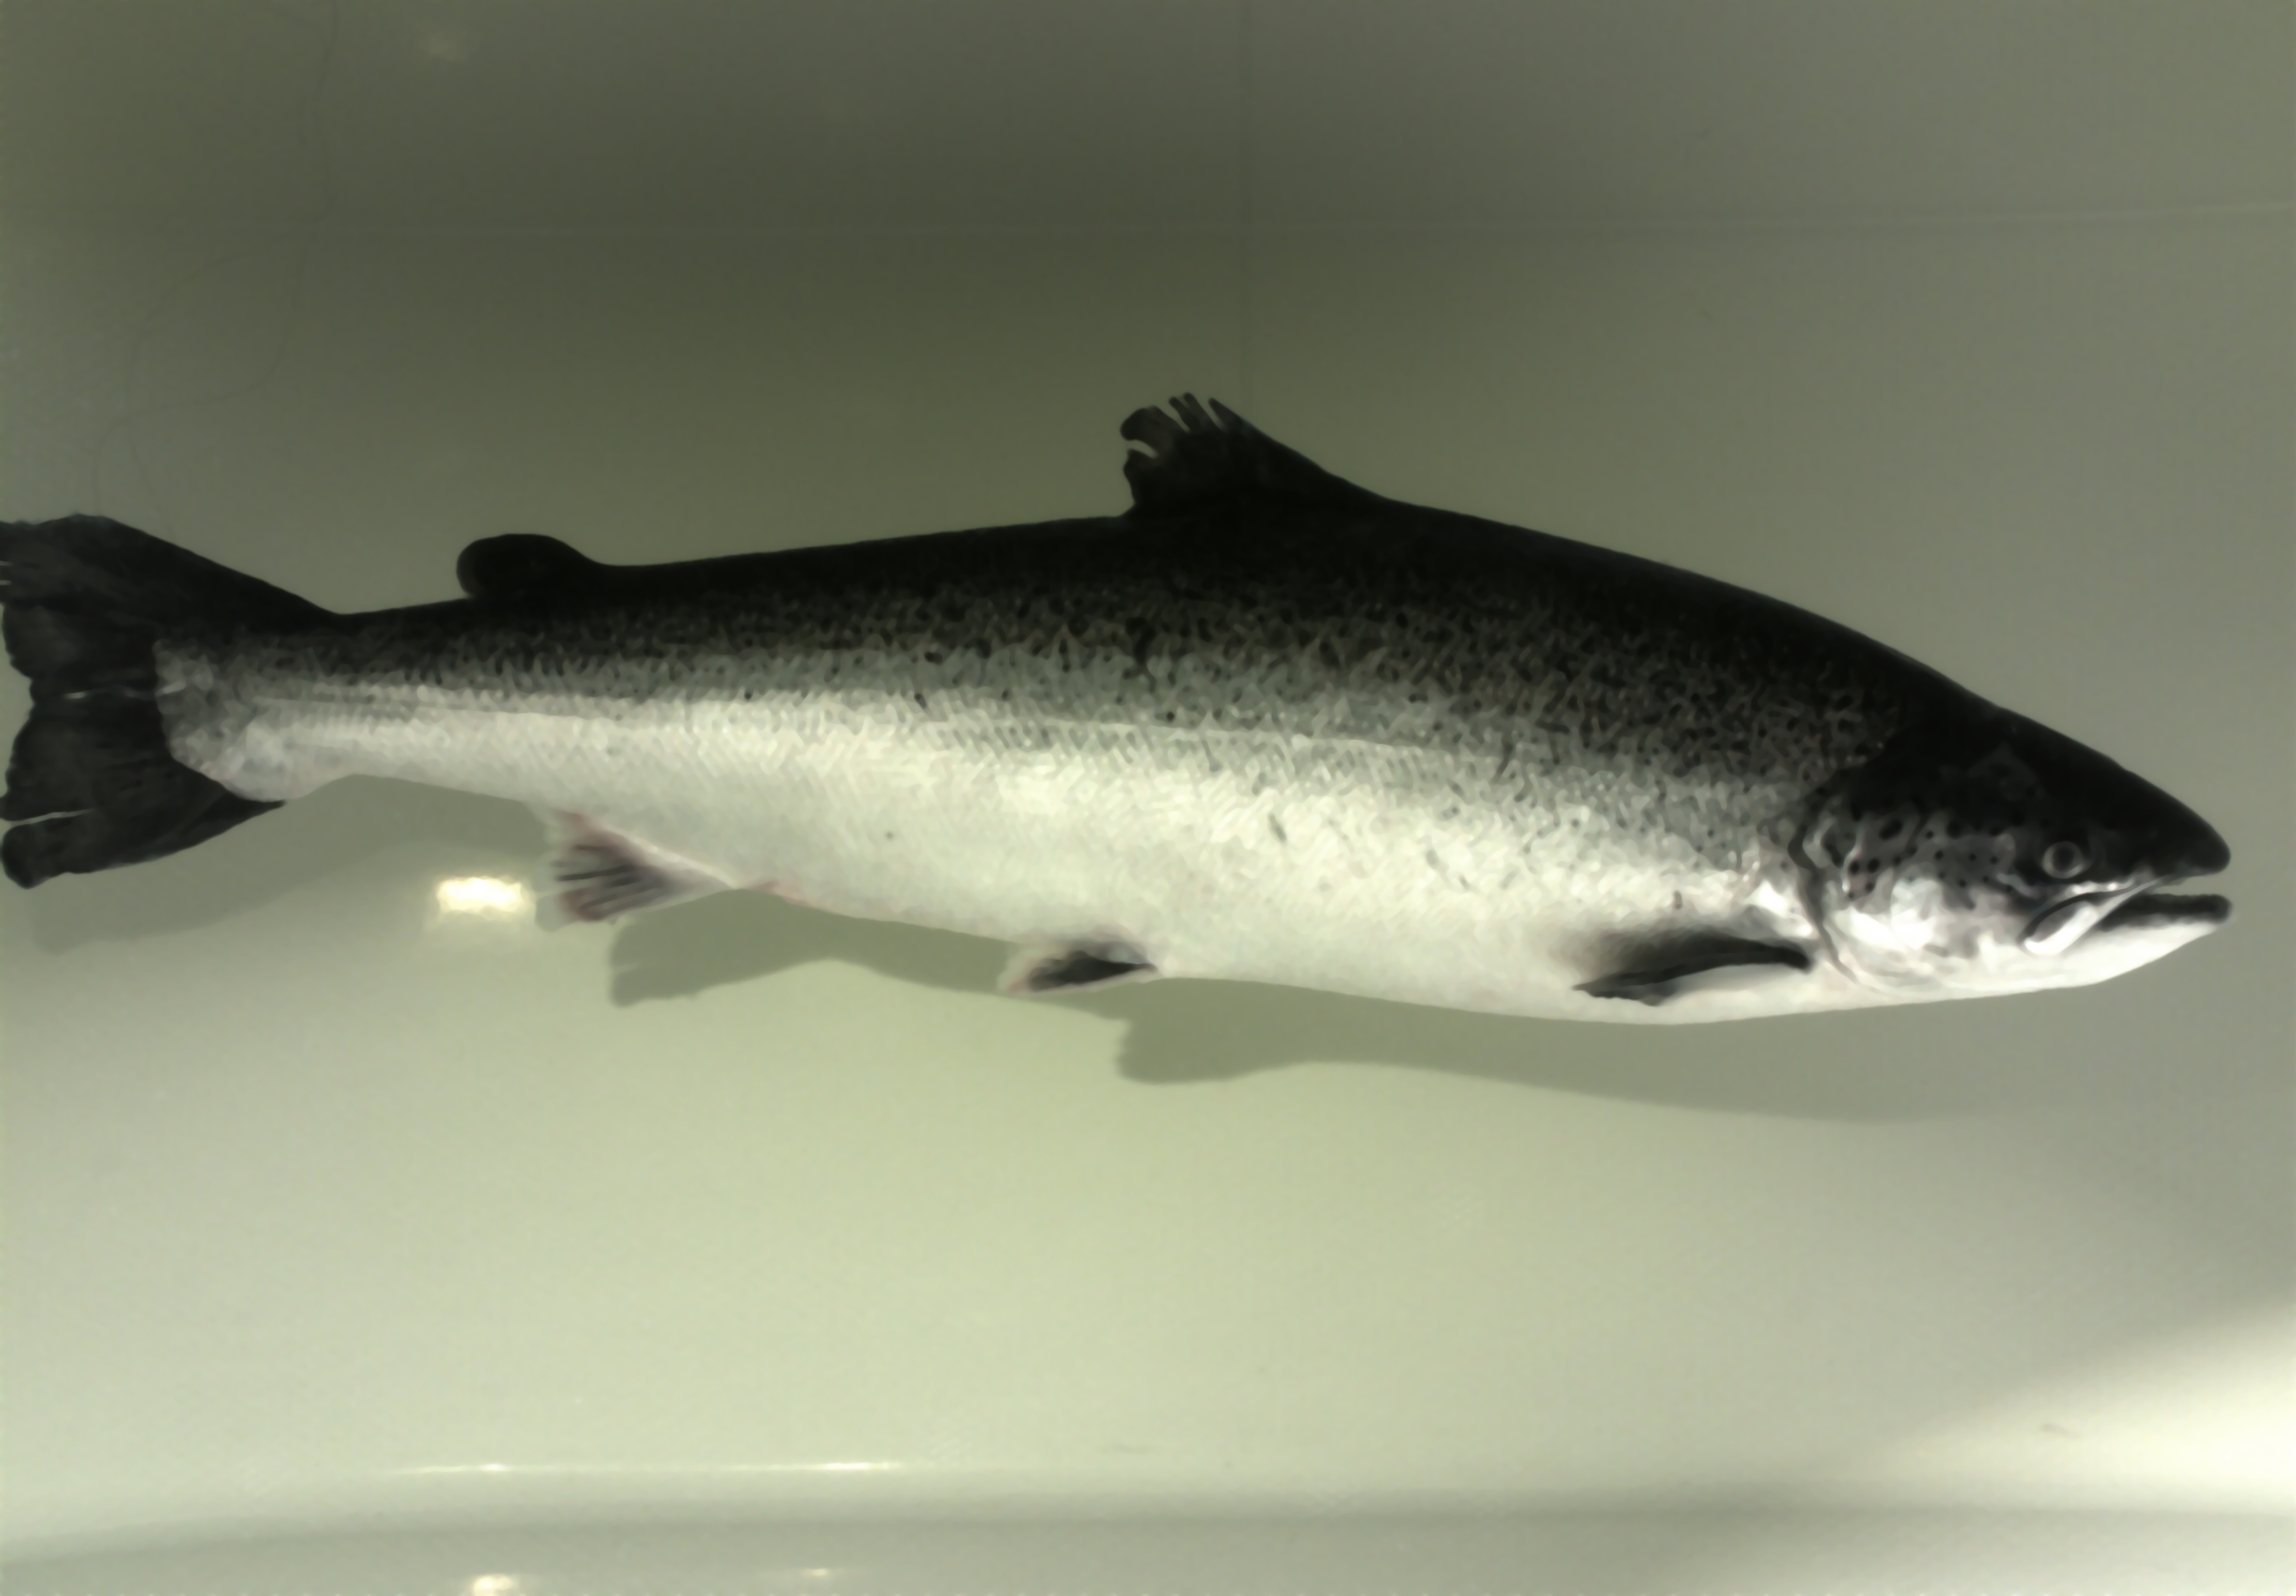
\includegraphics[width=.9\linewidth]{images/literature/median_filter}
        \caption{Bilateral Filter}
    \end{subfigure}
    \caption{Example of bilateral filtering}
    \label{fig:bilateral_filter}
\end{figure}

From figure \ref{fig:bilateral_filter} it is possible to see that the edges are well preserved while small particles are removed from the image. The image was filtered with kernel size {\color{red}????}, and it was filtered {\color{red}?????} times in a row.


\subsection{Shadow Removal}
Simple shadow removal can be done by transforming the color space of the image from RBG to HSV and then setting the value component of each pixel to a constant value. What this really does is even out all grey tones in the image, as is shown in figure \ref{fig:shadow_removal}.

\begin{figure}[h]
    \centering
    \begin{subfigure}{0.5\textwidth}
        \centering
        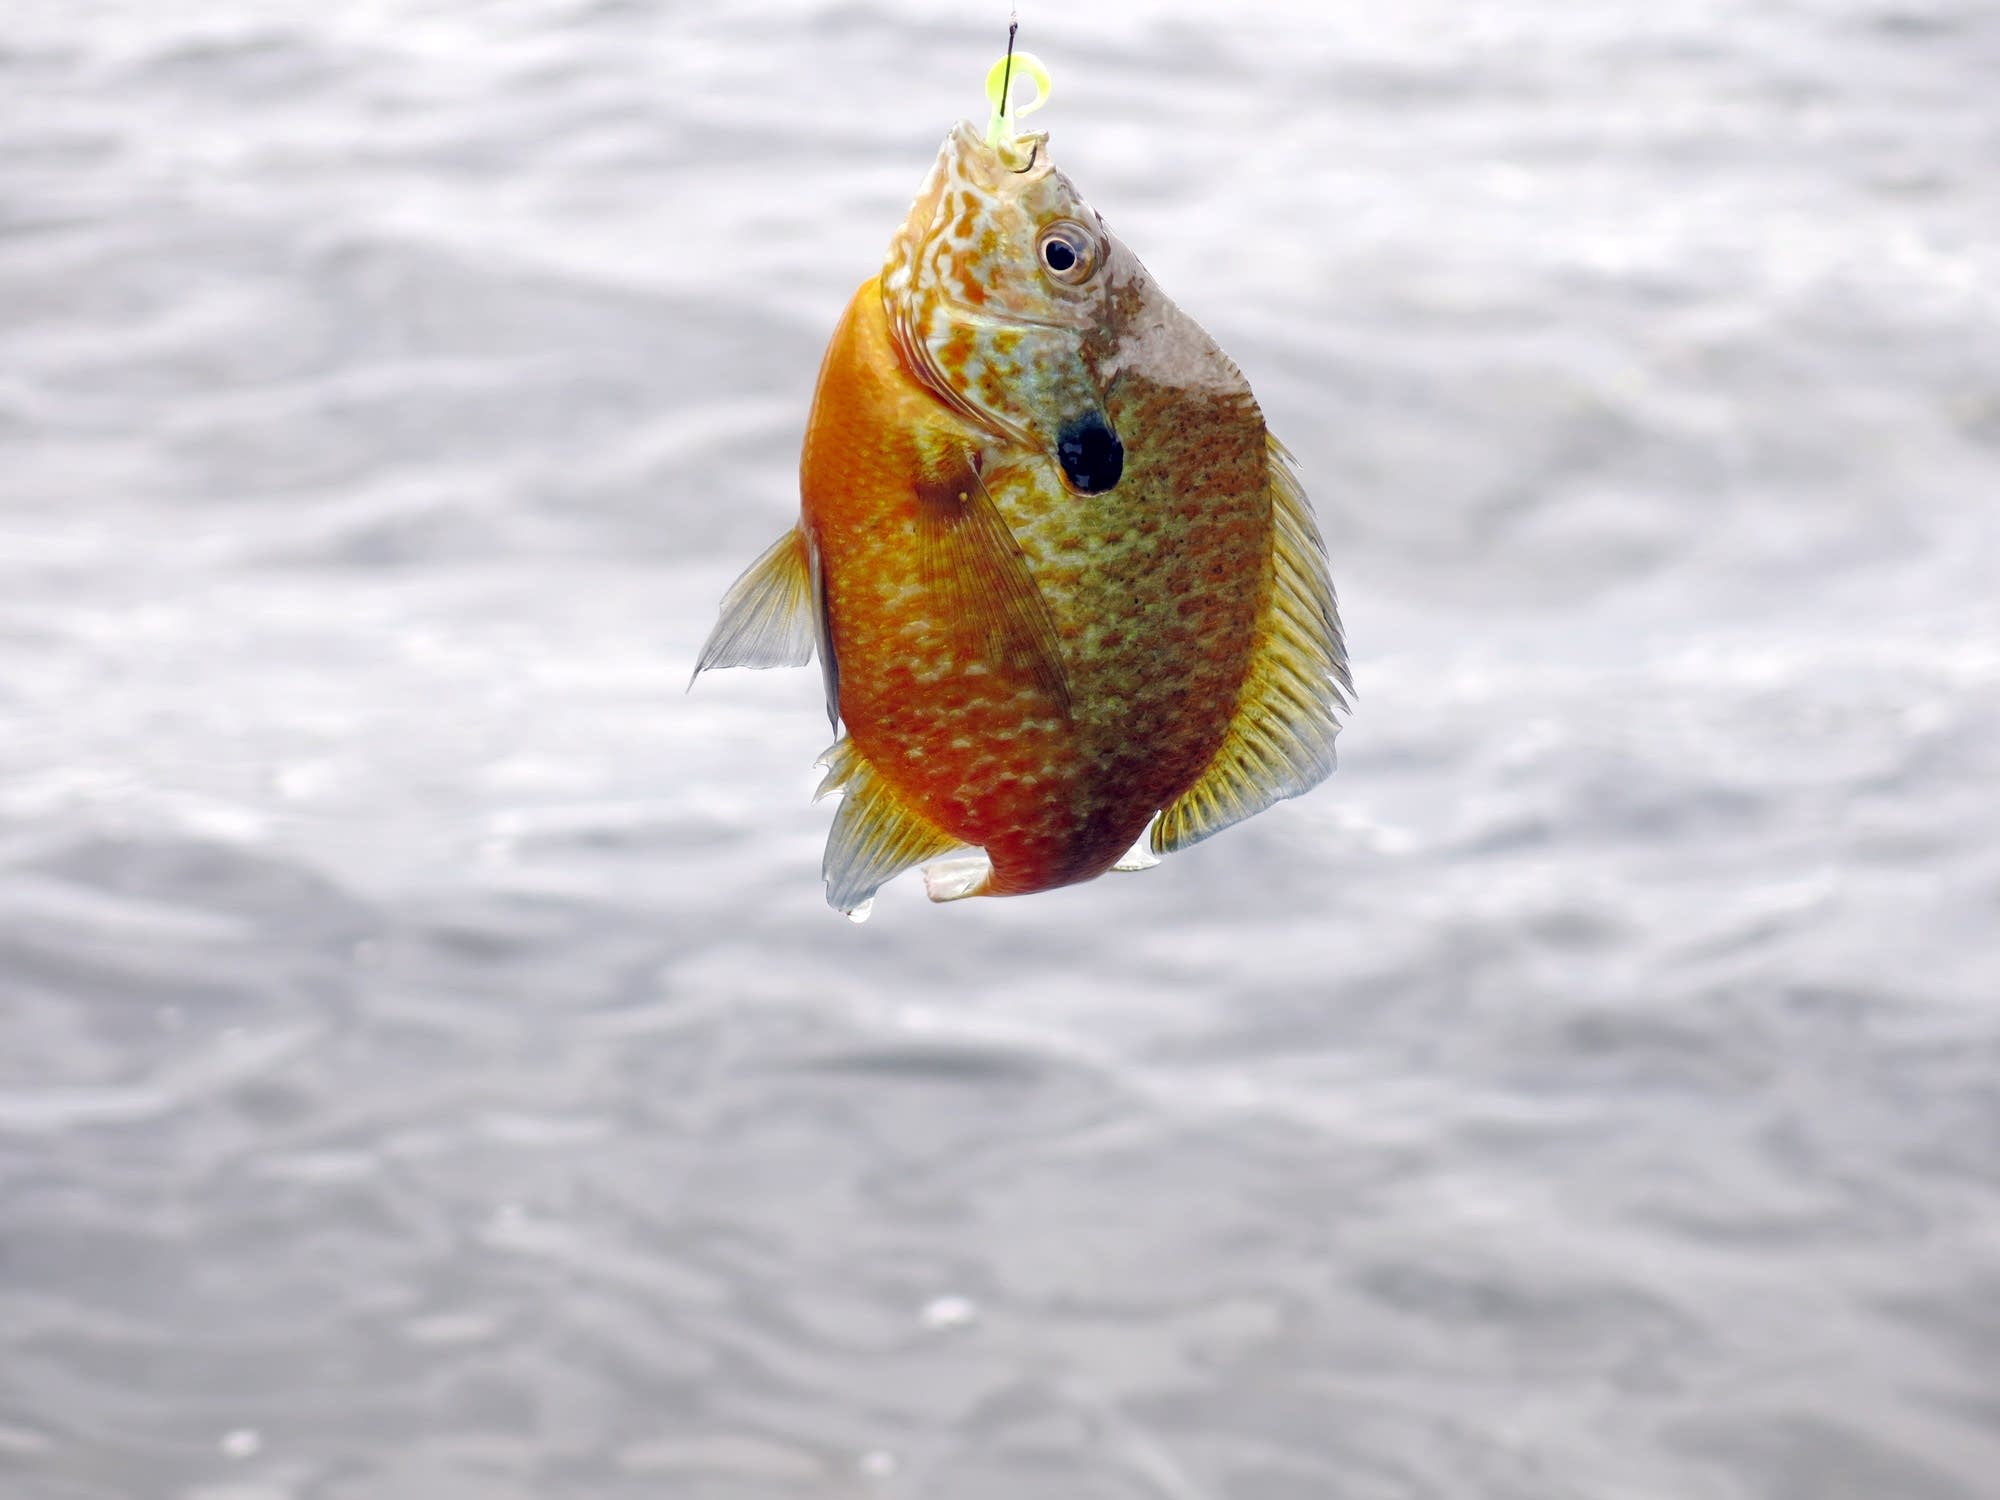
\includegraphics[width=.9\linewidth]{images/literature/colorfish}
        \caption{Original Image}
    \end{subfigure}%
    \begin{subfigure}{.5\textwidth}
        \centering
        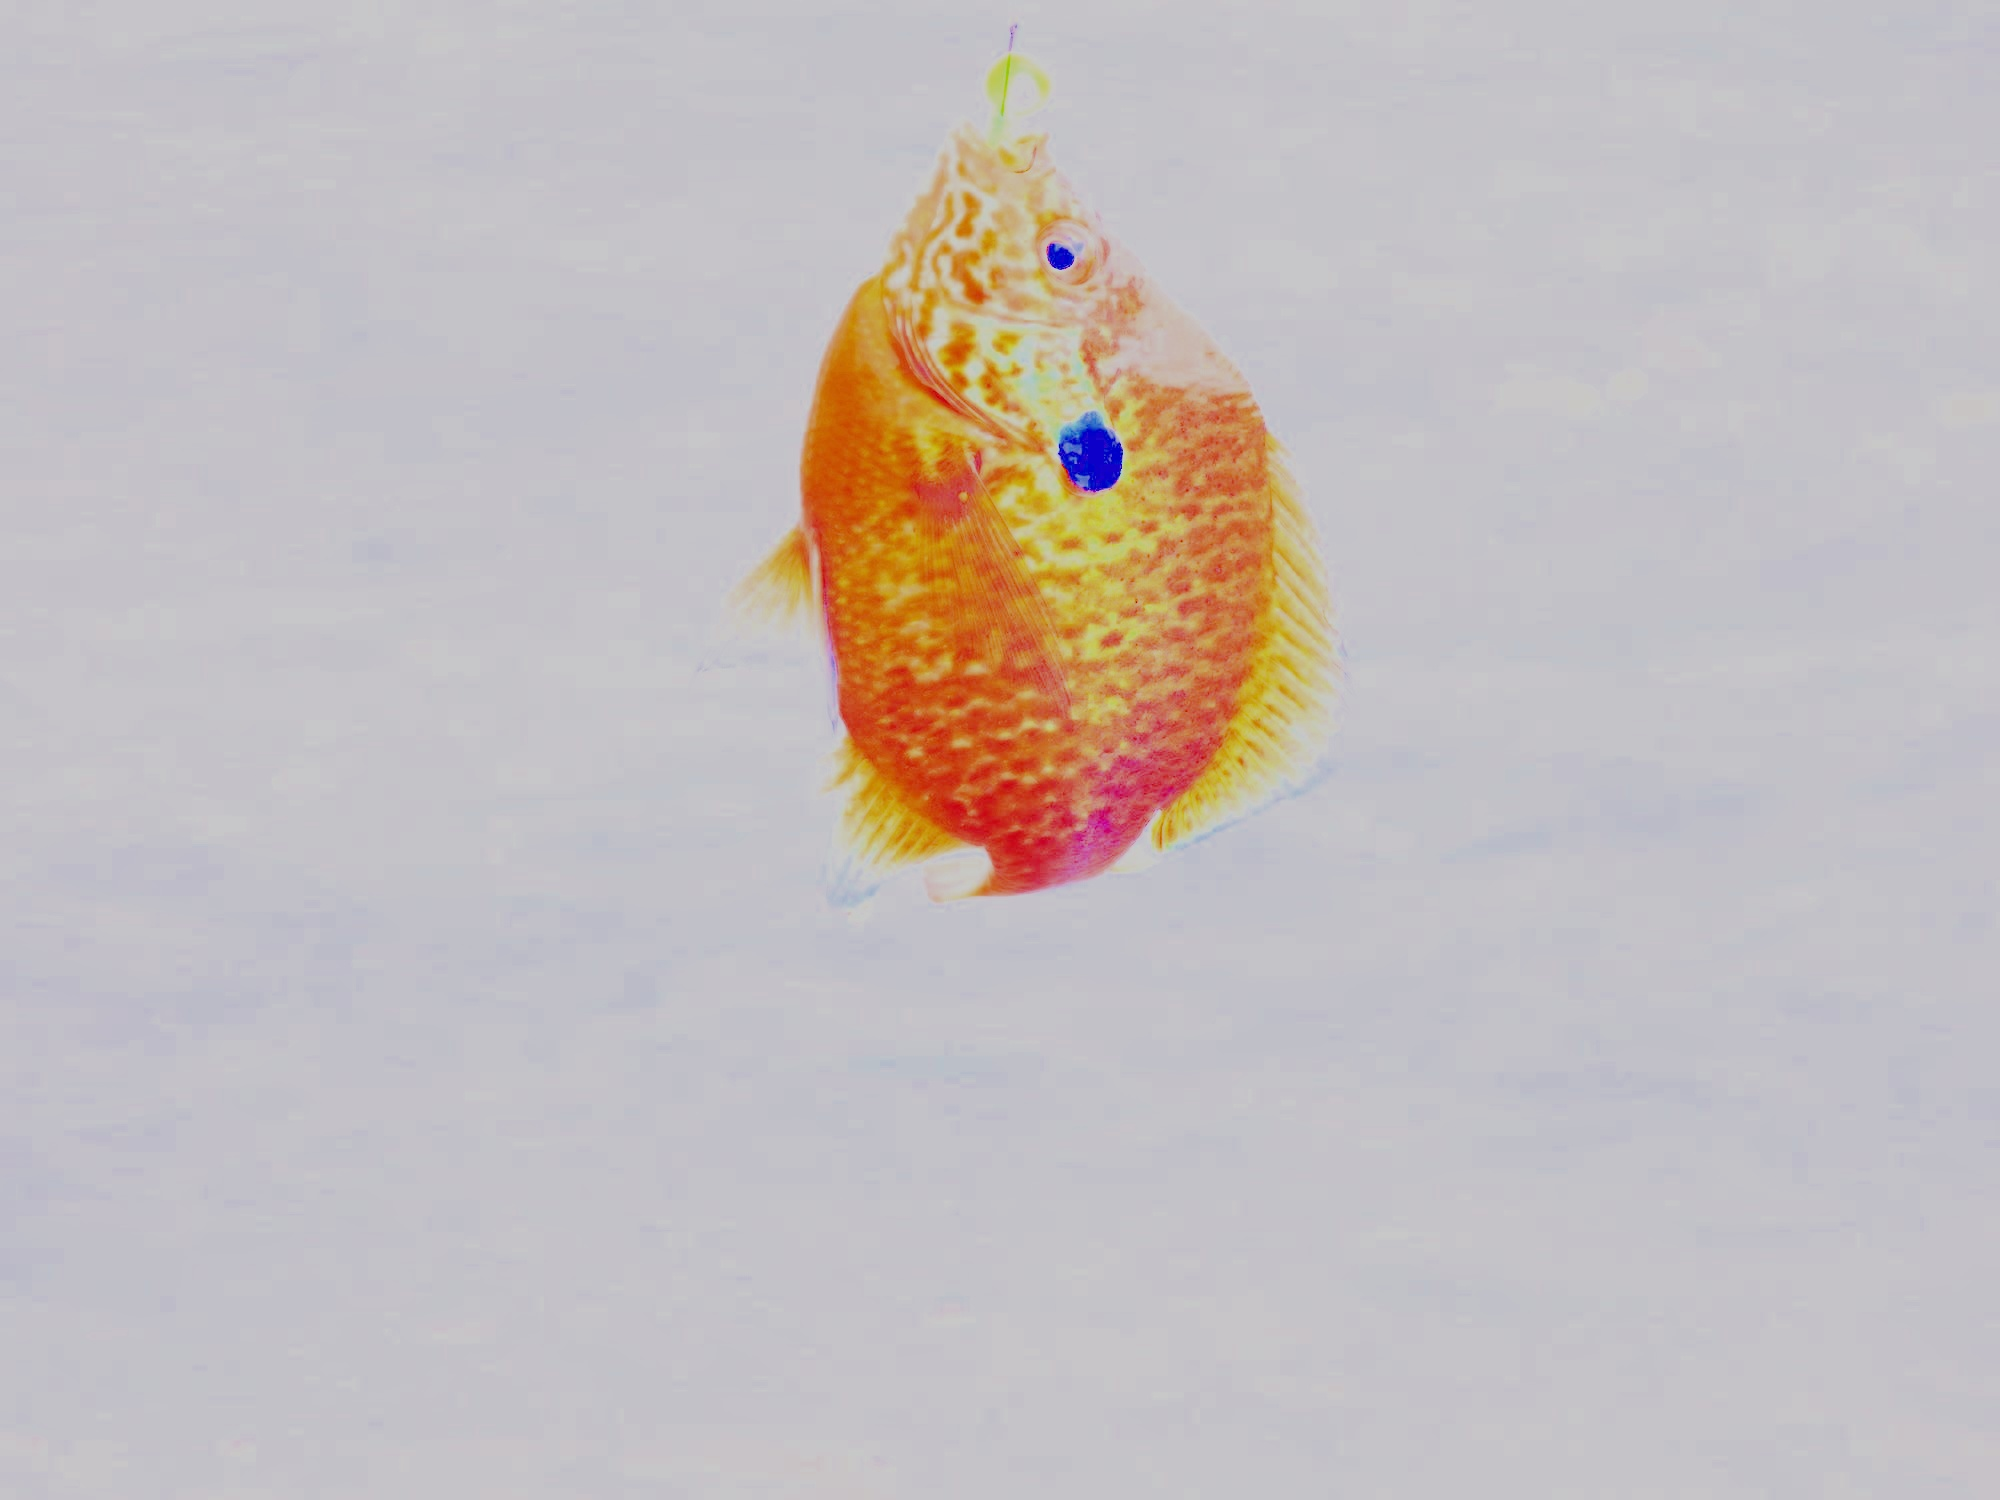
\includegraphics[width=.9\linewidth]{images/literature/shadow_removal}
        \caption{Shadow Removal}
    \end{subfigure}
    \caption{Example of shadow removal}
    \label{fig:shadow_removal}
\end{figure}

In figure \ref{fig:shadow_removal} it is shown that the colors of the fish is preserved, while all the shadows and blurry background in grey tones is evened out. In this example the value component is set to 200.

This type of simple shadow removal can be very useful, but for the image in figure \ref{fig:median_filter} the fish is not colorful enough for the technique to remove the shadows only.

%%%%%%%%%%%%%%%%%%%%%%%%%%%%%%%%%%%%%%%%%%%%%%%%%%%%%%%%%%%%%%%%%%%%%%

\subsection{Filtering in the Frequency Domain}

The frequency domain is a space in which the image value at some pixel represents the amount that the intensity values vary over some distance. Changes done in the frequency domain affects the rate at which the intensity values are changing in the spatial domain. 
The Fourier Transform is mostly used to convert images from the spatial domain into the frequency domain, and the Inverse Fourier Transform is used to convert the other way. 
Filtering in the frequency domain is mostly used for removing continuous patters that occur in the spatial domain image.
Filtering in the frequency domain is also faster than running an averaging filter in the spatial domain, especially as the kernel size increases. 

In the frequency domain the spectrum is used to see the amplitudes of the sinusoids. A large amplitude implies a pattern in the spatial image. By removing the wanted amplitudes from the spectrum and using the Inverse Fourier Transform, the pattern from the amplitudes will be removed.
By removing certain frequencies in the frequency domain it is possible to remove patters like stripes on old images or light scattering in underwater images.


\subsubsection{Light scattering}
There are many problems with underwater image processing due to the light propagation in the water medium. The physical properties of water cause degradation effects not present in images taken in air. The water absorbs light and therefore limits the visibility distance, and it also causes scattering, which changes the direction of the light path. This influences the overall performance of underwater imaging systems. Forward scattering is the spreading of light from an object towards the camera, while backward scattering is the light reflected by the water towards the camera before it actually reaches an object. Backward scattering reduces the contrast of the image, and is seen as sunbeams on the image. Scattering comes from not only the water, but all particles in the water. \cite{article:underwater_image_processing}

\begin{figure}[h]
    \centering
    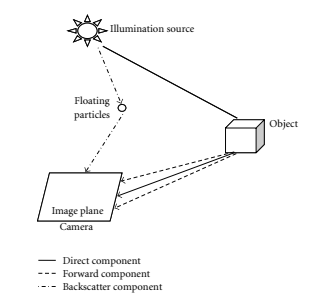
\includegraphics[width=0.7\textwidth]{images/image_from_paper}
    \caption{Explanation of scattering from (Raimondo Schettini and Silvia Corchs, 2010, p. 3)}
    \label{fig:image_from_paper}
\end{figure}

Filtering in the frequency domain could be a solution to reduce the scattering in underwater images.

%%%%%%%%%%%%%%%%%%%%%%%%%%%%%%%%%%%%%%%%%%%%%%%%%%%%%%%%%%%%%%%%%%%%%%

\subsection{Morphological Operators}

Morphology is a wide set of operations that process images based on shape. The operators apply a structuring element to an input image, and the value of each pixel in the output image is based on a comparison of the pixel with its neighbors. The structuring element is chosen by size and shape, and therefore determines what shapes the operation is sensitive towards. 
The shape of the structuring element can be chosen as flat or non-flat. Examples of flat structuring elements are ellipse, cross or rectangle, as shown below. Non-flat structuring elements have different weighting on the neighboring pixels. 

\noindent Ellipse: 
$\begin{bmatrix}
    0 & 0 & 1 & 0 & 0 \\
    0 & 1 & 1 & 1 & 0 \\
    1 & 1 & 1 & 1 & 1 \\
    0 & 1 & 1 & 1 & 0 \\
    0 & 0 & 1 & 0 & 0
\end{bmatrix}$ 
Cross: 
$\begin{bmatrix}
    0 & 0 & 1 & 0 & 0 \\
    0 & 0 & 1 & 0 & 0 \\
    1 & 1 & 1 & 1 & 1 \\
    0 & 0 & 1 & 0 & 0 \\
    0 & 0 & 1 & 0 & 0 
\end{bmatrix}$
Rect: 
$\begin{bmatrix}
    1 & 1 & 1 & 1 & 1 \\
    1 & 1 & 1 & 1 & 1 \\
    1 & 1 & 1 & 1 & 1 \\
    1 & 1 & 1 & 1 & 1 \\
    1 & 1 & 1 & 1 & 1
\end{bmatrix}$

Example of non-flat structuring element:
$\begin{bmatrix}
    0 & 0 & 1 & 0 & 0 \\
    0 & 1 & 2 & 1 & 0 \\
    1 & 2 & 4 & 2 & 1 \\
    0 & 1 & 2 & 1 & 0 \\
    0 & 0 & 1 & 0 & 0
\end{bmatrix}$ 

Morphological operators are useful for separating objects from each other, or merging objects together. It can also be used to remove small objects from an image, separate objects, merge objects, or to highlight certain objects.


\subsubsection{Dilate and Erode}
The most basic morphological operators are dilation and erosion. On gray-scale images dilation will add pixels on white object boundaries, while erosion will add pixels on black object boundaries.
\begin{itemize}
    \item Dilation: The value of the output pixel is the \textit{maximum} value of all pixels in the input pixels neighborhood. 
    \item Erosion: The value of the output pixel is the \textit{minimum} value of all pixels in the input pixels neighborhood. \cite{website:mathworks_dilation_erosion}
\end{itemize}

\begin{figure}[h]
    \centering
    \begin{subfigure}{0.33\textwidth}
        \centering
        
\includegraphics[width=.9\linewidth]{images/literature/star}
        \caption{Original Image}
    \end{subfigure}%
    \begin{subfigure}{.33\textwidth}
        \centering
        
\includegraphics[width=.9\linewidth]{images/literature/dilation}
        \caption{Dilation}
    \end{subfigure}%
    \begin{subfigure}{.33\textwidth}
        \centering
        
\includegraphics[width=.9\linewidth]{images/literature/erosion}
        \caption{Erosion}
    \end{subfigure}
    \caption{Example of dilation and erosion}
    \label{fig:star_dilate_erode}
\end{figure}



\subsubsection{Opening and Closing}
Opening and closing are combinations of dilation and erosion. Opening is the dilation of the erosion of an image, while closing is the erosion of the dilation of an image. 

\begin{figure}[h]
    \centering
    \begin{subfigure}{0.33\textwidth}
        \centering
        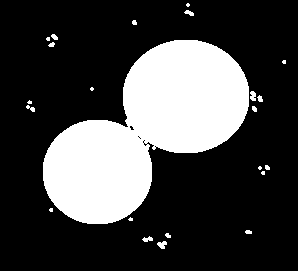
\includegraphics[width=.9\linewidth]{images/literature/dots}
        \caption{Original Image}
    \end{subfigure}%
    \begin{subfigure}{.33\textwidth}
        \centering
        
\includegraphics[width=.9\linewidth]{images/literature/opening}
        \caption{Opening}
    \end{subfigure}%
    \begin{subfigure}{.33\textwidth}
        \centering
        
\includegraphics[width=.9\linewidth]{images/literature/closing}
        \caption{Closing}
    \end{subfigure}
    \caption{Example of opening and closing}
    \label{fig:dots_opening_closing}
\end{figure}

Opening and closing assumes bright objects on a dark background. When opening an image, small objects will be removed and objects close to each other will be separated. When closing an image, objects close to each other will be closed together into one object. See figure \ref{fig:dots_opening_closing}.


%%%%%%%%%%%%%%%%%%%%%%%%%%%%%%%%%%%%%%%%%%%%%%%%%%%%%%%%%%%%%%%%%%%%%%


\clearpage

\section{Aim of the Study}\label{aim of study}

This section explains why the depthmap enhancement is needed, and how it would help the aquaculture industry. There is also a short section explaining the challenges met by working with the Raytrix camera and the depthmap images.

\subsection{Scope}

The goal of this project is to help SEALAB OCEAN GROUP on their way of making a complete camera system ready for underwater use for the aquaculture industry. SEALABs complete system should be able to detect the fish and classify it, measure the volume of the fish and detect salmon lice.
This projects focus is to better the depthmap images taken by the Raytrix camera so that the volume measurement becomes more accurate. Under the proper light conditions and at some certain distance, this individual system should be able to measure the volume of an object underwater. The task is aimed towards fish, especially salmon, as this system would mostly benefit the salmon breeding industry.
The aquaculture fish breeding industry is currently selling their fish without any knowledge on how much they actually got. With a complete camera system in place in every fish farm, an estimate of the total volume of fish can be made, salmon lice can be discovered earlier, and the companies can save huge amounts of money. 

The aim of this study is for the volume estimation of salmon to become more accurate. For this to happen, particles and unnecessary data needs to be removed and be replaced by relevant data. The depthmap computed by the Raytrix camera normally looks like the one in figure \ref{fig:depthmap82}, and it is seen from this image that there are holes in the fish, parts of the fish's belly and head is missing, and there are particles in front of the fish. This gives large opportunities for improvement, but also some challenges that need to be worked out.

\begin{figure}[H]
    \centering
    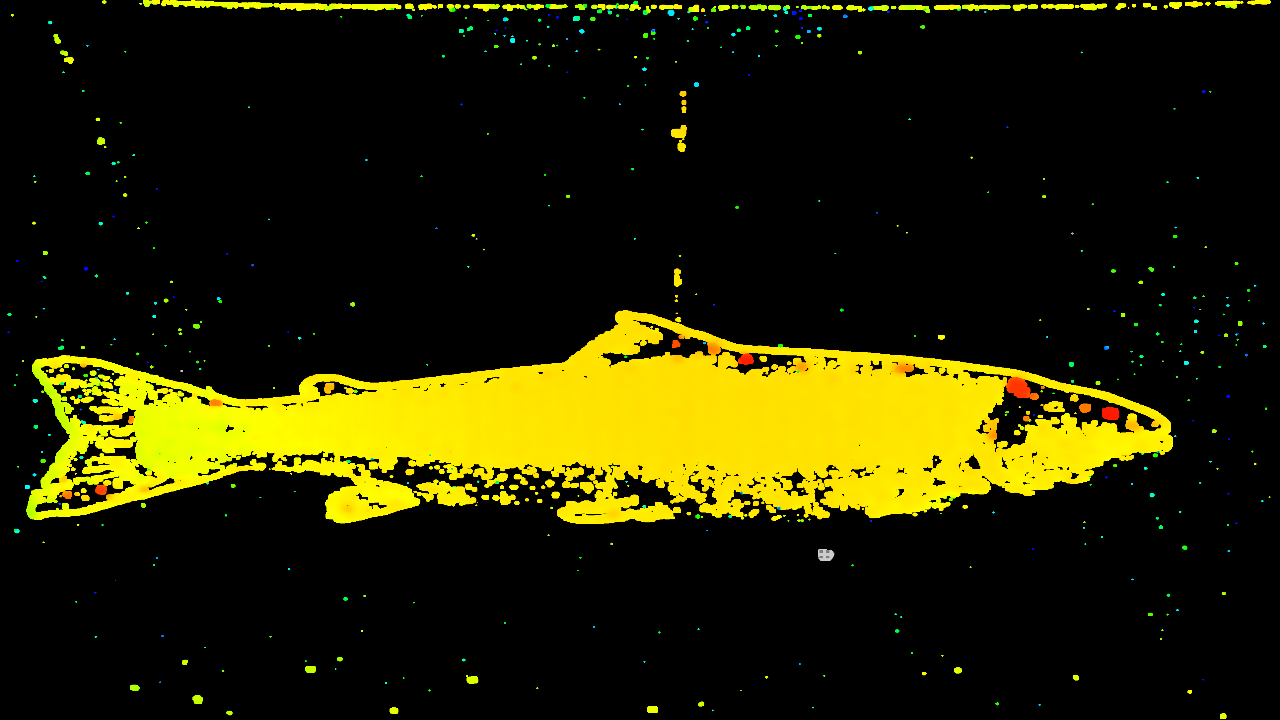
\includegraphics[width=.7\linewidth]{images/aim_of_study/depthmap82}
    \caption{Depthmap image of salmon}
    \label{fig:depthmap82}
\end{figure}


\subsection{Challenges}

The volume measurement is depending on the depth information stored in the depthmap image. For this measurement to be accurate, the data in the depthmap image must be more complete. Holes in the fish must be filled in while the shape of the fish remains.

A MATLAB 3D plot shows how insufficient the actual depth information is (see figure \ref{fig:matlab3D}). The particles make for large disturbances and the holes in the fish make for even bigger ones. The parts of the salmon that make for the largest depthmap errors is the belly, the fins and its head. The belly is white and the color is too close the the background color in the test facility. The head and fins are very black, and it could be a problem to the Raytrix that it is too black, and therefore makes it hard to see differences in each micro lens.

\begin{figure}[H]
    \centering
    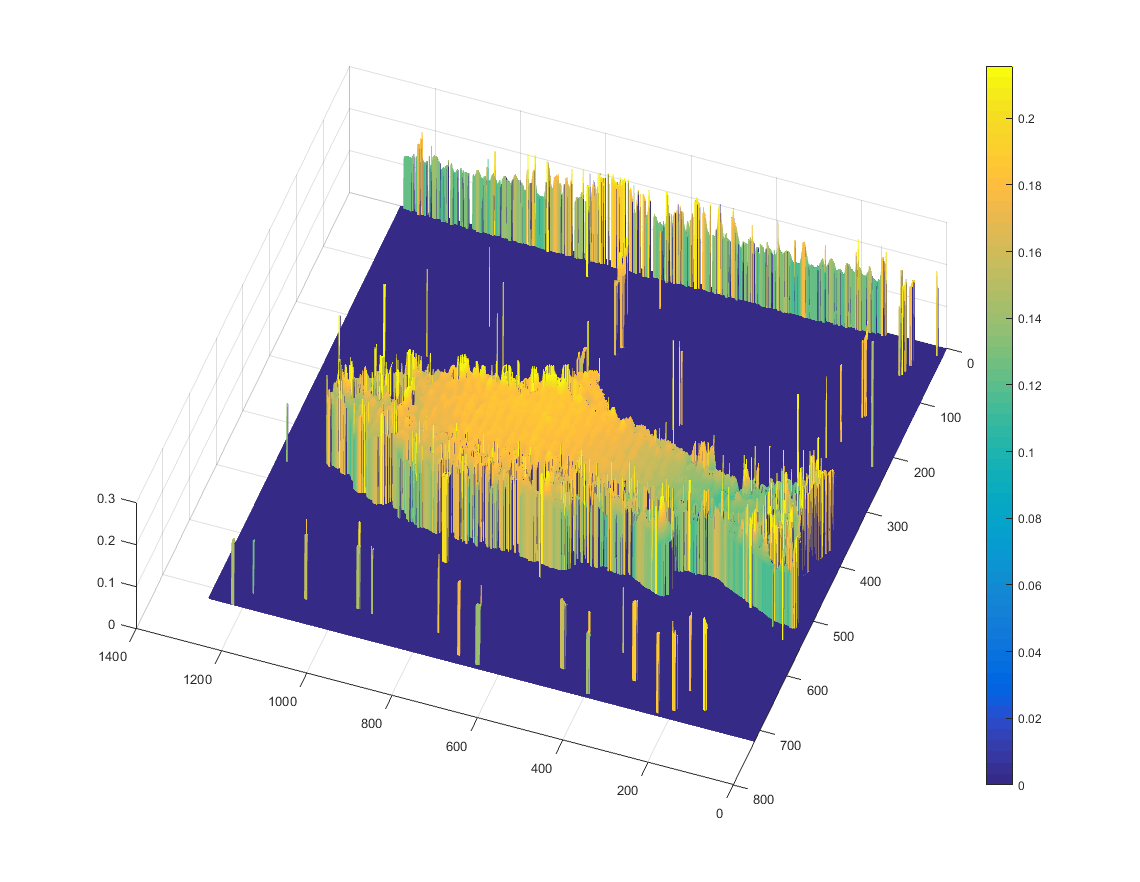
\includegraphics[width=.7\linewidth]{images/aim_of_study/original_3D_82}
    \caption{3D plot of depthmap}
    \label{fig:matlab3D}
\end{figure}

Even though there are many errors, it should be possible using the data from the depthmap image, enhance it and get a smooth surface of the fish, and thereby get a successful volume measurement. That is what the following sections in this report hope to show using the theory provided in section \ref{theory}.

\clearpage

\section{Methods and Implementation}\label{methods and implementation}

This section presents different processing techniques with the aim of solving the task at hand. Images will show the result, and the improvement is discussed. 

{\color{red}Explanation of kernel size, structuring element..????}

%%%%%%%%%%%%%%%%%%%%%%%%%%%%%%%%%%%%%%%%%%%%%%%%%%%%%%%%%%%%%%%%%%%%%%

\subsection{Median Filter}

%%%%%%%%%%%%%%%%%%%%%%%%%%%%%%%%%%%%%%%%%%%%%%%%%%%%%%%%%%%%%%%%%%%%%%

\subsection{Bilateral Filter}

%%%%%%%%%%%%%%%%%%%%%%%%%%%%%%%%%%%%%%%%%%%%%%%%%%%%%%%%%%%%%%%%%%%%%%

\subsection{Eroding and Dilating}
Erosion and dilation are two morphological operators. Eroding an image will enhance the black objects in an image, while dilating will enhance the white objects in an image. It uses a structuring element which decides how and how much the objects should change. 

%%%%%%%%%%%%%%%%%%%%%%%%%%%%%%%%%%%%%%%%%%%%%%%%%%%%%%%%%%%%%%%%%%%%%%

\subsection{Shadow Removal}

%%%%%%%%%%%%%%%%%%%%%%%%%%%%%%%%%%%%%%%%%%%%%%%%%%%%%%%%%%%%%%%%%%%%%%

\subsection{Fourier Filtering}

%%%%%%%%%%%%%%%%%%%%%%%%%%%%%%%%%%%%%%%%%%%%%%%%%%%%%%%%%%%%%%%%%%%%%%

\subsection{ACE}

%%%%%%%%%%%%%%%%%%%%%%%%%%%%%%%%%%%%%%%%%%%%%%%%%%%%%%%%%%%%%%%%%%%%%%

\subsection{Iqbal et al'. technique}

%%%%%%%%%%%%%%%%%%%%%%%%%%%%%%%%%%%%%%%%%%%%%%%%%%%%%%%%%%%%%%%%%%%%%%

\subsection{Histogram depth measurement}
\clearpage

\section{Experiments}\label{experiments}
In this section we describe the results.


\clearpage

\section{Conclusion}\label{conclusion}
We worked hard, and achieved very little.
\clearpage


\bibliographystyle{plain}
\bibliography{kilder}

\end{document}

  